\documentclass{beamer}
\usetheme{CambridgeUS}
\setbeamercolor{block title}{bg=red!80!black, fg=white}
\setbeamercolor{block body}{bg=red!10, fg=black}
%%%%%%%%%%%%%%%%%%%%%%%%%%%%%%%%%%%%%%%%%%%%%%%%%%%%%%%
\usepackage[utf8]{vietnam}
\usepackage{tikz}
% \usepackage{amsmath} % For mathematical environments
% \usepackage{cleveref} % For referencing
%%%%%%%%%%%%%%%%%%%%%%%%%%%%%%%%%%%%%%%%%%%%%%%%%%%%%%%
\usepackage[utf8]{vietnam}
\usepackage{tikz}

\usepackage{graphicx}
\usepackage{lipsum}
\usepackage{tikz}

\usepackage{bookmark}


\usepackage{hyperref}
\usepackage{amsmath}
\usepackage{amssymb}

% \usepackage{cleveref} % For referencing
%%%%%%%%%%%%%%%%%%%%%%%%%%%%%%%%%%%%%%%%%%%%%%%%%%%%%%%
\AtBeginSection[]
{
\begin{frame}<beamer>
\frametitle{Nội dung}

\tableofcontents[
currentsection,
subsectionstyle=hide/hide,
subsubsectionstyle=hide/hide
]
\end{frame}
}
%%%%%%%%%%%%%%%%%%%%%%%%%%%%%%%%%%%%%%%%%%%%%%%%%%%%%%%
\title[{\makebox[.15\paperwidth]{MI4100 - Mật mã và độ phức tạp thuật toán}}]{Chủ đề: Mô phỏng tấn công hệ mật mã khóa công khai RSA bằng thuật toán LLL giảm lưới}
\author[Nhóm 8]{Nhóm 8}
\date[\today]{\today}
%%%%%%%%%%%%%%%%%%%%%%%%%%%%%%%%%%%%%%%%%%%%%%%%%%%%%%%
\begin{document}
%%%%%%%%%%%%%%%%%%%%%%%%%%%%%%%%%%%%%%%%%%%%%%%%%%%%%%%
% % Trang tiêu đề cần có hình ảnh pictures/HUST2.jpeg
% % Không chỉnh sửa gì
% \begin{frame}
% \begin{tikzpicture}[remember picture, overlay]
% \node[anchor=center, inner sep=0pt] at (current page.center) {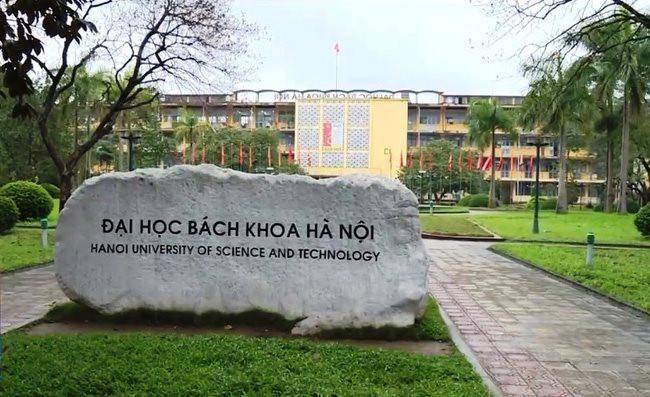
\includegraphics[width=\paperwidth, height=\paperheight]{pictures/HUST2.jpeg}};
% \fill[white, opacity=0.8] (current page.south west) rectangle (current page.north east);
% \end{tikzpicture}
% \titlepage
% \end{frame}
%%%%%%%%%%%%%%%%%%%%%%%%%%%%%%%%%%%%%%%%%%%%%%%%%%%%%%%
% \begin{frame}{Danh sách thành viên}
% \begin{block}{Nhóm 8}
% \centering
% \begin{tabular} {|l|c|}
% \hline
% Họ và tên & MSSV \\
% \hline
% Nguyễn Phan Anh & 20206113 \\
% Nguyễn Việt Anh & 20206115 \\
% Nguyễn Đình Anh & 20206111 \\
% Nguyễn Thị Hoa & 20206199 \\
% Vũ Văn Nghĩa & 20206205 \\
% \hline
% \end{tabular}
% \end{block}
% \end{frame}
%%%%%%%%%%%%%%%%%%%%%%%%%%%%%%%%%%%%%%%%%%%%%%%%%%%%%%%
% \begin{frame}{Phân công thành viên}
% \begin{block}{Phân công thành viên}
% \begin{itemize}
% \item Nguyễn Phan Anh: Lập kế hoạch, phân chia công việc, phân chia công việc, xxxxxxxxxxxxxxxxxxxxxxxxxxxxxx
% \item Nguyễn Việt Anh: Lập kế hoạch, phân chia công việc, phân chia công việc, xxxxxxxxxxxxxxxxxxxxxxxxxxxxxx
% \item Nguyễn Đình Anh: Lập kế hoạch, phân chia công việc, phân chia công việc, xxxxxxxxxxxxxxxxxxxxxxxxxxxxxx
% \item Nguyễn Thị Hoa: Lập kế hoạch, phân chia công việc, phân chia công việc, xxxxxxxxxxxxxxxxxxxxxxxxxxxxxx
% \item Vũ Văn Nghĩa: Lập kế hoạch, phân chia công việc, phân chia công việc, xxxxxxxxxxxxxxxxxxxxxxxxxxxxxx
% \end{itemize}
% \end{block}
% \end{frame}
%%%%%%%%%%%%%%%%%%%%%%%%%%%%%%%%%%%%%%%%%%%%%%%%%%%%%%%
%! %%%%%%%%%%%%%%%%%%%%%%%%%%%%%%%%%%%%%%%%%%%%%%%%%%%%%%
%! %%%%%%%%%%%%%%%%%%%%%%%%%%%%%%%%%%%%%%%%%%%%%%%%%%%%%%
%! %%%%%%%%%%%%%%%%%%%%%%%%%%%%%%%%%%%%%%%%%%%%%%%%%%%%%%
%! %%%%%%%%%%%%%%%%%%%%%%%%%%%%%%%%%%%%%%%%%%%%%%%%%%%%%%
%! %%%%%%%%%%%%%%%%%%%%%%%%%%%%%%%%%%%%%%%%%%%%%%%%%%%%%%
% \section{Tổng quan về hệ mật mã khóa công khai}
% \subsection{Lịch sử}
% \begin{frame}{Lịch sử}

% \begin{itemize}
% \item Hệ mật mã khóa công khai là một bước tiến lớn và là cuộc cách mạng trong lĩnh vực mật mã
% \item Hệ mật mã khóa công khai được Diffie và Hellman đưa ra năm 1976
% \end{itemize}

% \begin{columns}

% \begin{column}{0.4\textwidth}
% \begin{figure}[H]
% \centering
% 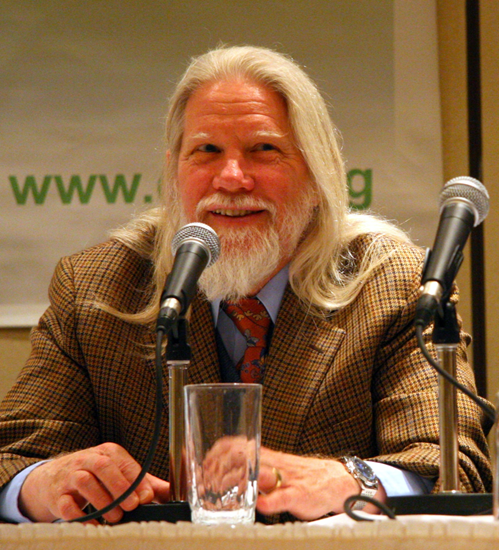
\includegraphics[scale = 0.4]{pictures/Bailey_Whitfield_Diffie.png}
% \end{figure}
% Bailey Whitfield 'Whit' Diffie\\ (sinh 05/06/1944 – 80 tuổi)
% \end{column}

% \begin{column}{0.4\textwidth}
% \begin{figure}[H]
% \centering
% 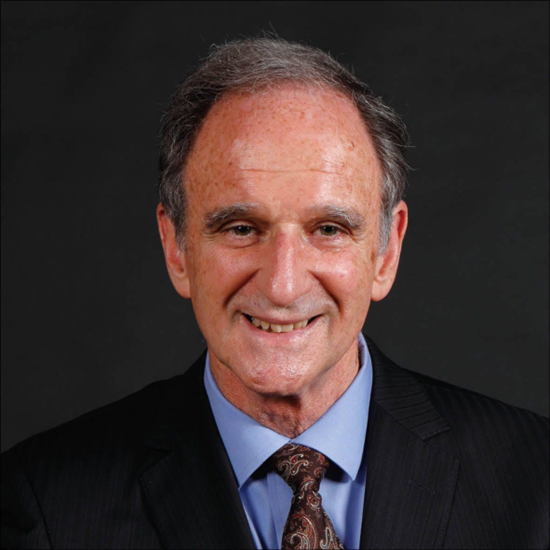
\includegraphics[scale = 0.4]{pictures/Martin_Edward_Hellman.png}
% \end{figure}
% Martin Edward Hellman\\(sinh 02/10/1945 - 79 tuổi)
% \end{column}

% \end{columns}
% \end{frame}
%%%%%%%%%%%%%%%%%%%%%%%%%%%%%%%%%%%%%%%%%%%%%%%%%%%%%%%
% \subsection{Khái niệm}
% \begin{frame}{Khái niệm}

% \begin{itemize}
% \item Hệ mật mã khóa công khai là một dạng mật mã hoá cho phép người sử dụng trao đổi các thông tin mật mà không cần phải trao đổi các khoá chung bí mật trước đó
% \item Việc mã hóa công khai được thực hiện bằng cách sử dụng một cặp khóa có quan hệ toán học với nhau là khóa công khai và khoá bí mật
% \begin{itemize}
% \item Khóa công khai: được công khai phổ biến - dùng để mã hóa
% \item Khóa bí mật: được giữ bí mật - dùng để giải mã
% \end{itemize}
% \end{itemize}

% $\Rightarrow$ Điều này đảm bảo hệ thống là không thể (hoặc rất khó) tìm ra khóa bí mật nếu chỉ biết khóa công khai

% \end{frame}
%%%%%%%%%%%%%%%%%%%%%%%%%%%%%%%%%%%%%%%%%%%%%%%%%%%%%%%
% \subsection{Mô hình tổng quát}
% \begin{frame}{Mô hình tổng quát}
% \begin{figure}[H]
% \centering
% 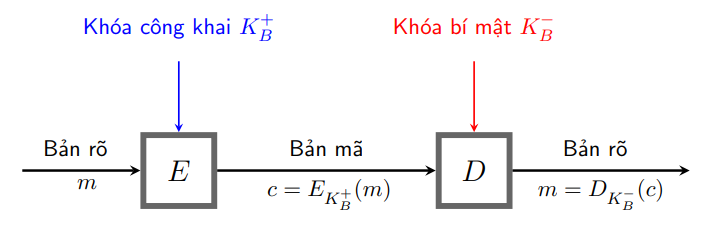
\includegraphics[scale = 0.6]{pictures/mo_hinh_tong_quat.png}
% \end{figure}

% \begin{block}{Nhận xét}
% Hệ mật mã khóa công khai được gọi là hệ mật mã bất đối xứng vì mã hóa và giải mã sử dụng khóa khác nhau
% \end{block}
% \end{frame}
%%%%%%%%%%%%%%%%%%%%%%%%%%%%%%%%%%%%%%%%%%%%%%%%%%%%%%%
% \subsection{Ưu, nhược điểm của hệ mã hóa công khai}
% \begin{frame}{Ưu điểm}
% \begin{itemize}
% \item Thuật toán được viết một lần, công khai cho nhiều lần dùng, cho nhiều người dùng, họ chỉ cần giữ bí mật khóa riêng của mình
% \item Khi biết các tham số ban đầu của hệ mã hóa, việc tính ra cặp khoá công khai và bí mật phải là "dễ", tức là trong thời gian đa thức
% \item Khả năng lộ khóa bí mật khó hơn vì chỉ có một người giữ gìn. Nếu thám mã biết khoá công khai, cố gắng tìm khoá bí mật, thì chúng phải đương đầu với bài toán "khó"
% \item Nếu thám mã biết khoá công khai và bản mã, thì việc tìm ra bản rõ cũng là bài toán "khó"
% \end{itemize}
% \end{frame}
%%%%%%%%%%%%%%%%%%%%%%%%%%%%%%%%%%%%%%%%%%%%%%%%%%%%%%%
% \begin{frame}{Nhược điểm}
% \begin{itemize}
% \item Hệ mã hóa khóa công khai: mã hóa và giải mã chậm hơn hệ mã hóa khóa bí mật
% \item Khả năng bị tấn công dạng tấn công người đứng giữa do kẻ tấn công lợi dụng việc phân phối khóa công khai để thay giả mạo gói tin
% \end{itemize}
% \end{frame}
%%%%%%%%%%%%%%%%%%%%%%%%%%%%%%%%%%%%%%%%%%%%%%%%%%%%%%%
% \subsection{So sánh với mã đối xứng}
% \begin{frame}{So sánh với mã đối xứng}

% \end{frame}
%%%%%%%%%%%%%%%%%%%%%%%%%%%%%%%%%%%%%%%%%%%%%%%%%%%%%%%
%! %%%%%%%%%%%%%%%%%%%%%%%%%%%%%%%%%%%%%%%%%%%%%%%%%%%%%%
%! %%%%%%%%%%%%%%%%%%%%%%%%%%%%%%%%%%%%%%%%%%%%%%%%%%%%%%
%! %%%%%%%%%%%%%%%%%%%%%%%%%%%%%%%%%%%%%%%%%%%%%%%%%%%%%%
%! %%%%%%%%%%%%%%%%%%%%%%%%%%%%%%%%%%%%%%%%%%%%%%%%%%%%%%
%! %%%%%%%%%%%%%%%%%%%%%%%%%%%%%%%%%%%%%%%%%%%%%%%%%%%%%%
% \section{Hệ mật mã RSA}
% \subsection{Tổng quan về hệ mật mã RSA}
% \begin{frame}{Tổng quan về hệ mật mã RSA}

% \begin{itemize}
% \item RSA là hệ mật mã khóa công khai phổ biến nhất trong thực tế, phát minh bởi Rivest, Shamir và Adleman (1977)
% \item Cơ sở thuật toán RSA dựa trên tính khó của bài toán phân tích các số lớn ra thừa số nguyên tố: không tồn tại thuật toán thời gian đa thức (theo độ dài của biểu diễn nhị phân của số đó) cho bài toán này.
% \end{itemize}

% \begin{figure}[H]
% \centering
% 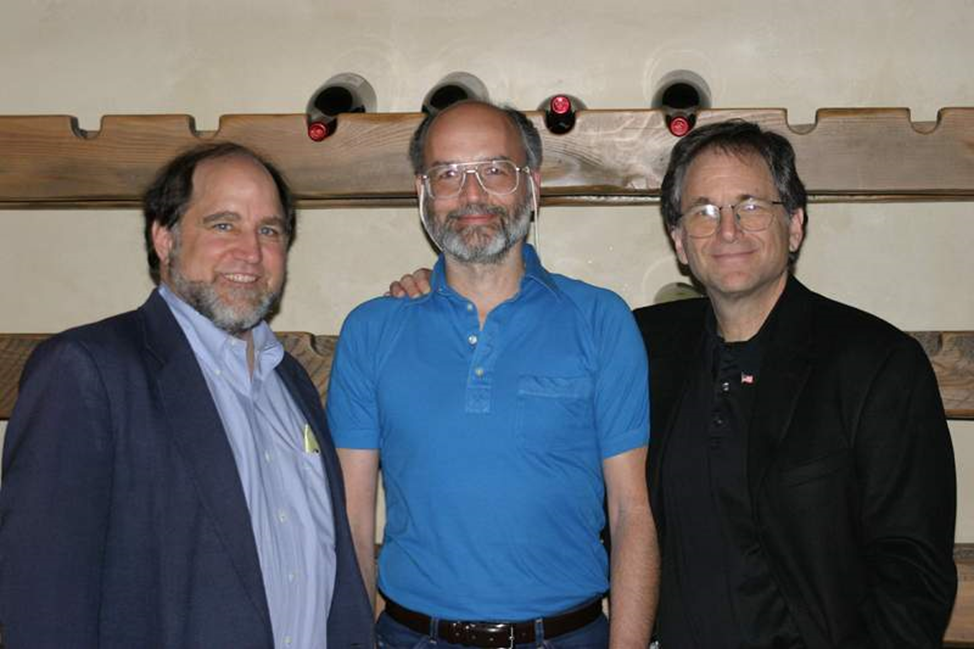
\includegraphics[scale = 0.4]{pictures/RSA_RonRivestAdiShamirLeonardAdleman.png}
% \end{figure}

% \end{frame}
%%%%%%%%%%%%%%%%%%%%%%%%%%%%%%%%%%%%%%%%%%%%%%%%%%%%%%%
% \subsection{Mã hóa và giải mã RSA}
% \begin{frame}{Mã hóa và giải mã RSA}
% \begin{itemize}
% \item Bảo mật của RSA dựa trên giả thuyết không có các thuật toán đủ nhanh để khai triển luỹ thừa một số. Qui trình áp dụng RSA gồm hai bước:
% \begin{enumerate}
% \item Lựa chọn (sinh) cặp khóa công khai và khóa bí mật
% \item Thực hiện thuật toán mã hoá và thuật toán giải mã
% \end{enumerate}
% \end{itemize}
% \end{frame}
%%%%%%%%%%%%%%%%%%%%%%%%%%%%%%%%%%%%%%%%%%%%%%%%%%%%%%%
% \begin{frame}{Thuật toán sinh khóa}

% \begin{enumerate}
% \item Chọn hai số nguyên tố đủ lớn, $p$ và $q$
% \item Tính toán $n = pq$ và $\phi(n) = (p - 1)(q - 1)$
% \item Chọn một số, $e$ $(1 < e < \phi(n))$ sao cho $\text{gcd}(e, \phi(n)) = 1$.

% Giá trị $e$ sẽ được sử dụng trong mã hoá
% \item Tìm một số $d$ sao cho $ed - 1$ chia hết cho $\phi(n)$, hay nói cách khác $d = e^{-1} \mod \phi(n)$. Giá trị $d$ sẽ được sử dụng để giải mã
% \item Công khai khóa $K^+_B$ = (n, e) và giữ bí mật khóa $K^-_B$ = (n, d)
% \end{enumerate}
% \end{frame}
%%%%%%%%%%%%%%%%%%%%%%%%%%%%%%%%%%%%%%%%%%%%%%%%%%%%%%%
% \begin{frame}{Mã hóa và giải mã RSA}
% \begin{itemize}
% \item Mã hóa:

% \[
% c = E (m, K_B^+) = m^e \mod n
% \]
% \item Giải mã:

% \[
% m = D (c, K_B^-) = c^d \mod n
% \]
% \end{itemize}
% \end{frame}
%%%%%%%%%%%%%%%%%%%%%%%%%%%%%%%%%%%%%%%%%%%%%%%%%%%%%%%
% \begin{frame}{Ví dụ về RSA}

% \begin{block}{Ví dụ}
% Cho bản rõ \(M = 15 \) sử dụng thuật toán RSA với \(p = 11 \), \(q = 3 \)
% \end{block}

% \textbf{Thuật toán sinh khóa:}

% \begin{itemize}
% \item Bước 1: \textbf{Với hai số nguyên tố}:
% $p = 11, \quad q = 3 \quad \Rightarrow \quad n = p \cdot q = 11 \cdot 3 = 33$
% \item Bước 2: \textbf{Tính hàm Euler}:
% \[
% \varphi(n) = (p - 1) \cdot (q - 1) = (11 - 1) \cdot (3 - 1) = 10 \cdot 2 = 20
% \]
% \item Bước 3: \textbf{Chọn số $e = 3$ nguyên tố cùng nhau với $\varphi(n) = 20$}
% \end{itemize}

% \end{frame}
%%%%%%%%%%%%%%%%%%%%%%%%%%%%%%%%%%%%%%%%%%%%%%%%%%%%%%%
% \begin{frame}{Ví dụ về RSA}

% \textbf{Thuật toán sinh khóa:}

% \begin{itemize}

% \item Bước 4: \textbf{Tính $d$ là nghịch đảo của $e$ trong modulo $\varphi(n)$}:
% \[
% d \cdot e \equiv 1 \pmod{20}
% \]
% Ta có:
% \[
% d \cdot 3 \equiv 1 \pmod{20} \quad \Rightarrow \quad d = 7 \quad \text{(theo thuật toán Euclid)}
% \]

% \item Bước 5: \textbf{Khóa công khai và khóa bí mật}:
% \begin{itemize}
% \item \textbf{Khóa công khai} $(K_B^+)$:
% \[
% (n, e) = (33, 3)
% \]
% \item \textbf{Khóa bí mật} $(K_B^-)$:
% \[
% (n, d) = (33, 7)
% \]
% \end{itemize}
% \end{itemize}
% \end{frame}
%%%%%%%%%%%%%%%%%%%%%%%%%%%%%%%%%%%%%%%%%%%%%%%%%%%%%%%
% \begin{frame}{Ví dụ về RSA}

% \begin{itemize}

% \item \textbf{Mã hóa bản rõ $M = 15$}:
% \[
% C = M^e \mod n = 15^3 \mod 33
% \]
% Tính toán:
% $15^3 = 3375 \Rightarrow C = 9$

% \item \textbf{Giải mã bản mã $C = 9$}:
% \[
% M = C^d \mod n = 9^7 \mod 33
% \]
% Tính toán:
% \[
% 9^2 = 81 \quad \Rightarrow \quad 81 \mod 33 = 15
% \]
% \[
% 9^4 = 15^2 = 225 \quad \Rightarrow \quad 225 \mod 33 = 24
% \]
% \[
% 9^7 = 9^{4+2+1} = 9^4 \cdot 9^2 \cdot 9 = 24 \cdot 15 \cdot 9 = 3240 \quad \Rightarrow \quad 3240 \mod 33 = 15
% \]
% \[
% \Rightarrow M = 15
% \]

% \end{itemize}
% \end{frame}
%%%%%%%%%%%%%%%%%%%%%%%%%%%%%%%%%%%%%%%%%%%%%%%%%%%%%%%
% \begin{frame}{Ví dụ về RSA}

% \textbf{Ví dụ lập trình RSA:}

% \begin{figure}[H]
% \centering
% 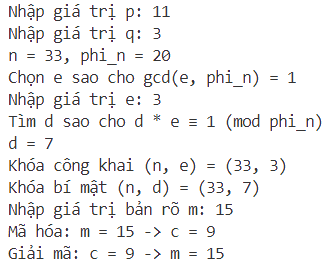
\includegraphics[scale = 1]{pictures/lap_trinh_vi_du_RSA.png}
% \end{figure}

% \end{frame}
%%%%%%%%%%%%%%%%%%%%%%%%%%%%%%%%%%%%%%%%%%%%%%%%%%%%%%%
%! %%%%%%%%%%%%%%%%%%%%%%%%%%%%%%%%%%%%%%%%%%%%%%%%%%%%%%
%! %%%%%%%%%%%%%%%%%%%%%%%%%%%%%%%%%%%%%%%%%%%%%%%%%%%%%%
%! %%%%%%%%%%%%%%%%%%%%%%%%%%%%%%%%%%%%%%%%%%%%%%%%%%%%%%
%! %%%%%%%%%%%%%%%%%%%%%%%%%%%%%%%%%%%%%%%%%%%%%%%%%%%%%%
%! %%%%%%%%%%%%%%%%%%%%%%%%%%%%%%%%%%%%%%%%%%%%%%%%%%%%%%
\section{Lý thuyết lưới}
\begin{frame}{Lý thuyết lưới}
\begin{itemize}
\item Lý thuyết lưới là một lĩnh vực trong toán học có liên quan đến việc nghiên cứu các cấu trúc đại số và hình học của các mạng lưới được phát triển từ những năm 1940.
\item Lý thuyết lưới được sử dụng trong nhiều lĩnh vực:
\begin{itemize}
\item Lĩnh vực mật mã học
\item Lĩnh vực khoa học máy tính
\item Lĩnh vực kỹ thuật thông tin
\end{itemize}
\end{itemize}
\end{frame}
%%%%%%%%%%%%%%%%%%%%%%%%%%%%%%%%%%%%%%%%%%%%%%%%%%%%%%%
% \subsection{Định nghĩa}
% \begin{frame}{Định nghĩa}
% \begin{block}{Tập hợp các vector độc lập tuyến tính}
% Tập hợp các vector \(\{x_1, x_2, \ldots, x_n\}\) trong \(\mathbb{R}^n\) độc lập tuyến tính nếu:
% \[
% c_1 x_1 + c_2 x_2 + \ldots + c_n x_n = 0 \text{với} c_i \in \mathbb{R}
% \]
% Dấu "=" xảy ra khi và chỉ khi \(c_1 = c_2 = \ldots = c_n = 0 \).
% \end{block}
% \end{frame}
%%%%%%%%%%%%%%%%%%%%%%%%%%%%%%%%%%%%%%%%%%%%%%%%%%%%%%%

%! %%%%%%%%%%%%%%%%%%%%%%%%%%%%%%%%%%%%%%%%%%%%%%%%%%%%%%
%! %%%%%%%%%%%%%%%%%%%%%%%%%%%%%%%%%%%%%%%%%%%%%%%%%%%%%%
%! %%%%%%%%%%%%%%%%%%%%%%%%%%%%%%%%%%%%%%%%%%%%%%%%%%%%%%
%! %%%%%%%%%%%%%%%%%%%%%%%%%%%%%%%%%%%%%%%%%%%%%%%%%%%%%%
%! %%%%%%%%%%%%%%%%%%%%%%%%%%%%%%%%%%%%%%%%%%%%%%%%%%%%%%
% \section{Tổng kết}
% \subsection{Tổng kết}
% \subsubsection{Tổng kết}
% \begin{frame}{Tổng kết}
%
% Trên đây là toàn văn báo cáo Đồ án 1 về chủ đề \textbf{Phương pháp lưới}. Trong đồ án này, em đã trình bày một số kiến thức cơ bản về lý thuyết lưới, tìm hiểu về thuật toán LLL và nhận thấy một phần tầm quan trọng của nó tróng lý thuyết số và mật mã.Trong bài báo cáo có giới thiệu về một số hệ mật mã như RSA và NTRU, thực hiện các cuộc tấn công vào chúng và thực hiện chạy chương trình thực nghiệm trên phần mềm SageMath.\\

% Báo
% cáo Đồ án vẫn còn rất nhiều thiếu sót, vậy nên em rất mong được thầy và các bạn đọc cùng
% góp ý, nhận xét để báo cáo trở nên hoàn thiện hơn.\\

% \end{frame}
%%%%%%%%%%%%%%%%%%%%%%%%%%%%%%%%%%%%%%%%%%%%%%%%%%%%%%%
%! %%%%%%%%%%%%%%%%%%%%%%%%%%%%%%%%%%%%%%%%%%%%%%%%%%%%%%
%! %%%%%%%%%%%%%%%%%%%%%%%%%%%%%%%%%%%%%%%%%%%%%%%%%%%%%%
%! %%%%%%%%%%%%%%%%%%%%%%%%%%%%%%%%%%%%%%%%%%%%%%%%%%%%%%
%! %%%%%%%%%%%%%%%%%%%%%%%%%%%%%%%%%%%%%%%%%%%%%%%%%%%%%%
%! %%%%%%%%%%%%%%%%%%%%%%%%%%%%%%%%%%%%%%%%%%%%%%%%%%%%%%
\section*{}
\begin{frame}{}
\centering
\Huge{Thanks for listening!}
\end{frame}
%%%%%%%%%%%%%%%%%%%%%%%%%%%%%%%%%%%%%%%%%%%%%%%%%%%%%%%
\end{document}

\begin{frame}
\frametitle{Công thức Toán học và Tham chiếu}
Xét công thức sau:
\begin{equation}
E = mc^2
\label{eq:einstein}
\end{equation}
Công thức \cref{eq:einstein} là công thức nổi tiếng của Einstein.
\end{frame}